\documentclass[11pt,a4paper]{article}

% Packages
\usepackage[utf8]{inputenc}
\usepackage[T1]{fontenc}
\usepackage{lmodern}
\usepackage[margin=1in]{geometry}
\usepackage{hyperref}
\usepackage{listings}
\usepackage{xcolor}
\usepackage{graphicx}
\usepackage{tikz}
\usetikzlibrary{shapes,arrows,positioning,fit,calc}
\usepackage{amsmath}
\usepackage{booktabs}
\usepackage{enumitem}
\usepackage{fancyhdr}
\usepackage{tocloft}
\usepackage{tabularx}

% Hyperref setup
\hypersetup{
    colorlinks=true,
    linkcolor=blue,
    filecolor=magenta,
    urlcolor=cyan,
}

% Code listing style
\definecolor{codebg}{RGB}{245,245,245}
\definecolor{codegreen}{RGB}{0,128,0}
\definecolor{codegray}{RGB}{128,128,128}
\definecolor{codepurple}{RGB}{128,0,128}
\definecolor{tsblue}{RGB}{0,122,204}

\lstdefinestyle{tscode}{
    backgroundcolor=\color{codebg},
    basicstyle=\ttfamily\small,
    breakatwhitespace=false,
    breaklines=true,
    captionpos=b,
    commentstyle=\color{codegreen},
    keywordstyle=\color{tsblue}\bfseries,
    numberstyle=\tiny\color{codegray},
    stringstyle=\color{codepurple},
    showstringspaces=false,
    numbers=left,
    numbersep=5pt,
    frame=single,
    rulecolor=\color{black},
    tabsize=2,
    morekeywords={interface,type,const,async,await,export,import,from,extends,implements}
}

\lstset{style=tscode}

% Header/Footer
\pagestyle{fancy}
\fancyhf{}
\rhead{BetterSys Architecture}
\lhead{Frontend-Backend Integration}
\rfoot{Page \thepage}

% Title
\title{%
    \textbf{BetterSys: Frontend-Backend Integration} \\
    \large Communication Patterns, Data Flow, and Synchronization
}
\author{System Documentation}
\date{January 2026}

\begin{document}

\maketitle
\tableofcontents
\newpage

%==============================================================================
\section{Architecture Overview}
%==============================================================================

BetterSys employs a hybrid communication architecture combining REST API polling with WebSocket streaming for real-time signal delivery. The frontend is built with React 18 and TypeScript, using Zustand for state management.

\subsection{Technology Stack}

\begin{table}[h]
\centering
\begin{tabular}{@{}llll@{}}
\toprule
\textbf{Layer} & \textbf{Frontend} & \textbf{Backend} & \textbf{Protocol} \\
\midrule
Runtime & Vite + React 18 & Tokio async & --- \\
State & Zustand & parking\_lot & --- \\
REST & fetch API & Axum handlers & HTTP/JSON \\
Streaming & WebSocket API & Axum WS & WS/JSON \\
Auth & localStorage JWT & JWT middleware & Bearer token \\
\bottomrule
\end{tabular}
\caption{Communication Stack}
\end{table}

\subsection{High-Level Data Flow}

\begin{figure}[h]
\centering
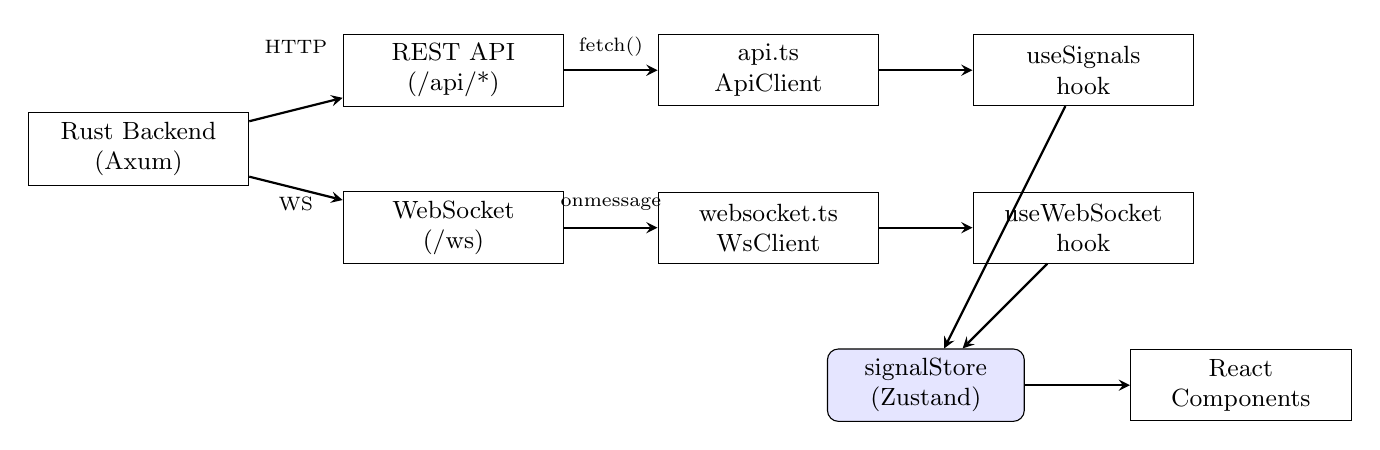
\begin{tikzpicture}[
    node distance=1.5cm,
    box/.style={rectangle, draw, minimum width=2.8cm, minimum height=0.9cm, align=center, font=\small},
    store/.style={rectangle, draw, rounded corners, minimum width=2.5cm, minimum height=0.8cm, align=center, fill=blue!10, font=\small},
    arrow/.style={->, thick, >=stealth},
    dasharrow/.style={->, thick, dashed, >=stealth},
]
    % Backend
    \node[box] (backend) at (0,0) {Rust Backend\\(Axum)};
    
    % Communication
    \node[box] (rest) at (4,1) {REST API\\(/api/*)};
    \node[box] (ws) at (4,-1) {WebSocket\\(/ws)};
    
    % Frontend Services
    \node[box] (apits) at (8,1) {api.ts\\ApiClient};
    \node[box] (wsts) at (8,-1) {websocket.ts\\WsClient};
    
    % Hooks
    \node[box] (usesig) at (12,1) {useSignals\\hook};
    \node[box] (usews) at (12,-1) {useWebSocket\\hook};
    
    % Store
    \node[store] (store) at (10,-3) {signalStore\\(Zustand)};
    
    % Components
    \node[box] (ui) at (14,-3) {React\\Components};
    
    % Arrows
    \draw[arrow] (backend) -- (rest);
    \draw[arrow] (backend) -- (ws);
    \draw[arrow] (rest) -- (apits);
    \draw[arrow] (ws) -- (wsts);
    \draw[arrow] (apits) -- (usesig);
    \draw[arrow] (wsts) -- (usews);
    \draw[arrow] (usesig) -- (store);
    \draw[arrow] (usews) -- (store);
    \draw[arrow] (store) -- (ui);
    
    % Labels
    \node[font=\scriptsize] at (2,1.3) {HTTP};
    \node[font=\scriptsize] at (2,-0.7) {WS};
    \node[font=\scriptsize] at (6,1.3) {fetch()};
    \node[font=\scriptsize] at (6,-0.7) {onmessage};
\end{tikzpicture}
\caption{Frontend-Backend Communication Architecture}
\end{figure}

%==============================================================================
\section{REST API Communication}
%==============================================================================

\subsection{API Client (api.ts)}

The frontend uses a singleton \texttt{ApiClient} class that manages authentication tokens and provides typed methods for all backend endpoints.

\begin{lstlisting}[caption={API Client Core Structure}]
class ApiClient {
  private token: string | null = null;
  private cachedHeaders: Record<string, string> | null = null;

  setToken(token: string | null) {
    this.token = token;
    this.cachedHeaders = null; // Invalidate cache
    if (token) {
      localStorage.setItem('betterbot_token', token);
    } else {
      localStorage.removeItem('betterbot_token');
    }
  }

  private getHeaders(): Record<string, string> {
    if (this.cachedHeaders) return this.cachedHeaders;
    const token = this.getToken();
    this.cachedHeaders = {
      'Content-Type': 'application/json',
      ...(token ? { 'Authorization': `Bearer ${token}` } : {}),
    };
    return this.cachedHeaders;
  }

  private async fetch<T>(
    endpoint: string,
    options: RequestInit = {},
    timeoutMs: number = 15_000
  ): Promise<T>;
}

export const api = new ApiClient();
\end{lstlisting}

\subsection{Endpoint Mapping}

\begin{table}[h]
\centering
\small
\begin{tabularx}{\textwidth}{@{}llXl@{}}
\toprule
\textbf{Frontend Method} & \textbf{Backend Endpoint} & \textbf{Purpose} & \textbf{Timeout} \\
\midrule
\texttt{login()} & POST /api/auth/login & JWT authentication & 15s \\
\texttt{getSignals()} & GET /api/signals & Signal list with context & 15s \\
\texttt{searchSignals()} & GET /api/signals/search & FTS5 full-history search & 15s \\
\texttt{getSignalEnrich()} & GET /api/signals/enrich & 15m Up/Down live data & 2s \\
\texttt{getMarketSnapshot()} & GET /api/market/snapshot & Orderbook snapshot & 2s \\
\texttt{getWalletAnalytics()} & GET /api/wallet/analytics & Performance curves & 10-20s \\
\texttt{getVaultState()} & GET /api/vault/state & Vault NAV/shares & 15s \\
\texttt{vaultDeposit()} & POST /api/vault/deposit & Mint shares & 5s \\
\texttt{vaultWithdraw()} & POST /api/vault/withdraw & Burn shares & 5s \\
\texttt{placeTradeOrder()} & POST /api/trade/order & One-click trade & 2.5s \\
\bottomrule
\end{tabularx}
\caption{Frontend-to-Backend API Mapping}
\end{table}

\subsection{Request/Response Flow}

\begin{lstlisting}[caption={Signal Fetching with Typed Response}]
// Frontend request
async getSignals(params?: {
  limit?: number;
  before?: string;
  before_id?: string;
  exclude_updown?: boolean;
}): Promise<{ signals: Signal[]; count: number; timestamp: string }> {
  const query = new URLSearchParams();
  if (params?.limit) query.set('limit', params.limit.toString());
  // ... build query string
  return this.fetch(`/api/signals?${query.toString()}`);
}

// Backend handler (Rust)
pub async fn get_signals_simple(
  Query(params): Query<SignalQuery>,
  AxumState(state): AxumState<AppState>,
) -> Json<SignalResponse> {
  // Fetch from SQLite, merge contexts, return JSON
}
\end{lstlisting}

%==============================================================================
\section{WebSocket Communication}
%==============================================================================

\subsection{Connection Lifecycle}

The WebSocket client handles connection, authentication, auto-reconnect, and message routing:

\begin{lstlisting}[caption={WebSocket Client Implementation}]
export class WebSocketClient {
  private ws: WebSocket | null = null;
  private reconnectAttempts = 0;
  private maxReconnectAttempts = 5;
  private reconnectDelay = 1000;

  connect() {
    const token = localStorage.getItem('betterbot_token');
    // Token passed as query param (WS doesn't support headers)
    const wsUrl = token ? `${WS_URL}?token=${token}` : WS_URL;
    
    this.ws = new WebSocket(wsUrl);
    
    this.ws.onopen = () => {
      this.reconnectAttempts = 0;
      this.emit('status', 'connected');
      this.startPing();
    };

    this.ws.onmessage = (event) => {
      const message = JSON.parse(event.data);
      this.handleMessage(message);
    };

    this.ws.onclose = () => {
      this.emit('status', 'disconnected');
      this.attemptReconnect();
    };
  }
}
\end{lstlisting}

\subsection{Message Types}

\begin{table}[h]
\centering
\begin{tabular}{@{}llp{7cm}@{}}
\toprule
\textbf{Type} & \textbf{Direction} & \textbf{Payload} \\
\midrule
\texttt{signal} & Server $\rightarrow$ Client & New \texttt{MarketSignal} object \\
\texttt{signal\_context} & Server $\rightarrow$ Client & Enrichment update for existing signal \\
\texttt{ping} & Client $\rightarrow$ Server & \texttt{\{timestamp: number\}} \\
\texttt{pong} & Server $\rightarrow$ Client & Echo of ping timestamp for latency \\
\bottomrule
\end{tabular}
\caption{WebSocket Message Protocol}
\end{table}

\subsection{Backend WebSocket Handler}

\begin{lstlisting}[caption={Rust WebSocket Handler},language=Rust]
async fn handle_socket(mut socket: WebSocket, state: AppState) {
  let mut rx = state.signal_broadcast.subscribe();

  // Replay recent signals on connect
  if let Ok(recent) = state.signal_storage.get_recent(200) {
    for signal in recent {
      let msg = serde_json::to_string(&WsServerEvent::Signal(signal))?;
      socket.send(Message::Text(msg)).await?;
    }
  }

  loop {
    tokio::select! {
      // Broadcast new signals
      Ok(event) = rx.recv() => {
        let msg = serde_json::to_string(&event)?;
        socket.send(Message::Text(msg)).await?;
      }
      // Handle client messages
      Some(Ok(msg)) = socket.recv() => {
        if let Message::Text(text) = msg {
          if text.contains("ping") {
            // Echo pong with timestamp
            socket.send(Message::Text(pong_json)).await?;
          }
        }
      }
    }
  }
}
\end{lstlisting}

\subsection{Signal Replay on Connect}

When a WebSocket connection is established, the backend immediately replays up to 200 recent signals. This ensures the UI is populated even if the REST polling hasn't completed:

\begin{enumerate}
    \item Client connects to \texttt{/ws?token=<JWT>}
    \item Backend validates token via \texttt{auth\_middleware}
    \item Backend fetches recent signals from SQLite
    \item Backend sends each signal as a \texttt{signal} message
    \item Backend sends stored context for each signal
    \item Client \texttt{addSignals()} merges into Zustand store
\end{enumerate}

%==============================================================================
\section{State Management}
%==============================================================================

\subsection{Zustand Signal Store}

The frontend maintains a single source of truth for signals using Zustand:

\begin{lstlisting}[caption={Signal Store Structure}]
interface SignalStore {
  signals: Signal[];
  stats: SignalStats | null;
  isLoading: boolean;
  error: string | null;
  
  addSignal: (signal: Signal) => void;
  addSignals: (signals: Signal[]) => void;
  applySignalContextUpdate: (update: SignalContextUpdate) => void;
  setSignals: (signals: Signal[]) => void;
  setStats: (stats: SignalStats) => void;
  clearSignals: () => void;
  setError: (error: string | null) => void;
}

export const useSignalStore = create<SignalStore>((set) => ({
  signals: [],
  // ... implementation
}));
\end{lstlisting}

\subsection{Signal Merging Strategy}

REST and WebSocket deliver signals with different context richness. The store merges them intelligently:

\begin{lstlisting}[caption={Signal Merge Logic}]
function mergeSignal(existing: Signal, incoming: Signal): Signal {
  // Compare context_version to determine which context is newer
  const existingCv = existing.context_version ?? -1;
  const incomingCv = incoming.context_version ?? -1;

  let preferExistingCtx = existingCv > incomingCv;

  // When versions equal, keep richer context
  if (existingCv === incomingCv) {
    preferExistingCtx = contextRichness(existing.context) 
                      > contextRichness(incoming.context);
  }

  return {
    ...existing,
    ...incoming,
    context: preferExistingCtx ? existing.context : incoming.context,
    context_version: Math.max(existingCv, incomingCv),
  };
}
\end{lstlisting}

\subsection{24-Hour Sliding Window}

The store maintains a bounded history to prevent memory growth:

\begin{lstlisting}[caption={History Trimming}]
const HISTORY_WINDOW_MS = 24 * 60 * 60 * 1000;  // 24 hours
const MAX_SIGNALS = 20_000;

function trimSignalsToWindow(signals: Signal[]): Signal[] {
  const cutoff = Date.now() - HISTORY_WINDOW_MS;
  const filtered = signals.filter((s) => {
    const t = Date.parse(s.detected_at);
    return Number.isNaN(t) || t >= cutoff;
  });
  return filtered.slice(0, MAX_SIGNALS);
}
\end{lstlisting}

%==============================================================================
\section{Polling and Synchronization}
%==============================================================================

\subsection{Adaptive Polling Strategy}

The \texttt{useSignals} hook adjusts polling frequency based on WebSocket health:

\begin{lstlisting}[caption={Adaptive Polling in useSignals}]
export const useSignals = (opts?: { wsConnected?: boolean }) => {
  useEffect(() => {
    loadSignals();
    loadStats();

    // Reduce polling when WS is connected (WS delivers real-time)
    const signalPollMs = opts?.wsConnected ? 5_000 : 500;
    const signalInterval = setInterval(loadSignals, signalPollMs);
    const statsInterval = setInterval(loadStats, 10_000);

    return () => {
      clearInterval(signalInterval);
      clearInterval(statsInterval);
    };
  }, [loadSignals, loadStats, opts?.wsConnected]);
};
\end{lstlisting}

\begin{table}[h]
\centering
\begin{tabular}{@{}lll@{}}
\toprule
\textbf{Condition} & \textbf{Signal Poll Rate} & \textbf{Rationale} \\
\midrule
WebSocket connected & 5 seconds & WS delivers real-time updates \\
WebSocket disconnected & 500ms & Compensate for lost streaming \\
Stats polling & 10 seconds & Stats are less time-sensitive \\
\bottomrule
\end{tabular}
\caption{Polling Rate Strategy}
\end{table}

\subsection{WebSocket Signal Buffering}

To prevent UI thrashing during rapid signal replay, signals are batched:

\begin{lstlisting}[caption={WebSocket Signal Buffering}]
const handleSignal = (signal: Signal) => {
  // Buffer signals to batch state updates
  signalBufferRef.current.push(signal);
  
  if (flushTimerRef.current == null) {
    flushTimerRef.current = window.setTimeout(() => {
      const batch = signalBufferRef.current;
      signalBufferRef.current = [];
      flushTimerRef.current = null;
      addSignals(batch);  // Single state update for batch
    }, 50);  // 50ms batching window
  }
};
\end{lstlisting}

%==============================================================================
\section{Authentication Flow}
%==============================================================================

\subsection{JWT Authentication Sequence}

\begin{figure}[h]
\centering
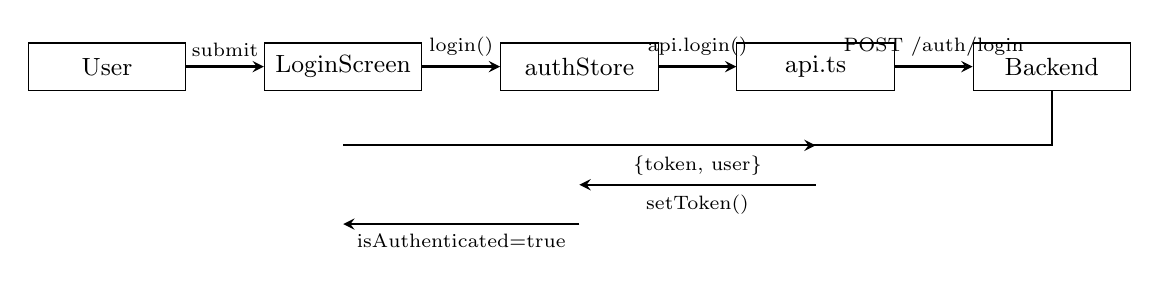
\begin{tikzpicture}[
    node distance=0.8cm,
    box/.style={rectangle, draw, minimum width=2cm, minimum height=0.6cm, align=center, font=\small},
    arrow/.style={->, thick, >=stealth},
]
    \node[box] (user) at (0,0) {User};
    \node[box] (login) at (3,0) {LoginScreen};
    \node[box] (auth) at (6,0) {authStore};
    \node[box] (api) at (9,0) {api.ts};
    \node[box] (backend) at (12,0) {Backend};
    
    \draw[arrow] (user) -- node[above, font=\scriptsize] {submit} (login);
    \draw[arrow] (login) -- node[above, font=\scriptsize] {login()} (auth);
    \draw[arrow] (auth) -- node[above, font=\scriptsize] {api.login()} (api);
    \draw[arrow] (api) -- node[above, font=\scriptsize] {POST /auth/login} (backend);
    
    \draw[arrow] (backend) -- ++(0,-1) -- node[below, font=\scriptsize] {\{token, user\}} ++(-9,0) -- (api |- 0,-1);
    \draw[arrow] (api |- 0,-1.5) -- node[below, font=\scriptsize] {setToken()} (auth |- 0,-1.5);
    \draw[arrow] (auth |- 0,-2) -- node[below, font=\scriptsize] {isAuthenticated=true} (login |- 0,-2);
\end{tikzpicture}
\caption{Authentication Sequence Diagram}
\end{figure}

\subsection{Auth Store Implementation}

\begin{lstlisting}[caption={Auth Store with Token Validation}]
export const useAuthStore = create<AuthStore>((set) => ({
  user: null,
  token: api.getToken(),
  isAuthenticated: false,
  
  login: async (username, password) => {
    set({ isLoading: true, error: null });
    const response = await api.login({ username, password });
    set({
      user: response.user,
      token: response.token,
      isAuthenticated: true,
    });
  },

  validateToken: async () => {
    const token = api.getToken();
    if (!token) {
      set({ isAuthenticated: false });
      return;
    }
    
    try {
      const response = await api.getCurrentUser();
      set({ user: response.user, isAuthenticated: true });
    } catch {
      api.logout();
      set({ isAuthenticated: false });
    }
  },
}));

// Auto-validate on store creation
if (api.getToken()) {
  useAuthStore.getState().validateToken();
}
\end{lstlisting}

\subsection{Protected Routes}

The \texttt{AuthGuard} component enforces authentication:

\begin{lstlisting}[caption={Auth Guard Component}]
export const AuthGuard: React.FC<{ children: ReactNode }> = ({ children }) => {
  const { isAuthenticated, isLoading } = useAuth();

  if (isLoading) {
    return <LoadingSpinner />;
  }

  if (!isAuthenticated) {
    return <LoginScreen />;
  }

  return <>{children}</>;
};
\end{lstlisting}

%==============================================================================
\section{Type Synchronization}
%==============================================================================

\subsection{Shared Type Definitions}

Frontend TypeScript types mirror backend Rust types exactly:

\begin{lstlisting}[caption={TypeScript Signal Type (matches Rust)}]
export type SignalType =
  | { type: 'PriceDeviation'; market_price: number; fair_value: number; 
      deviation_pct: number }
  | { type: 'MarketExpiryEdge'; hours_to_expiry: number; 
      volume_spike: number }
  | { type: 'WhaleFollowing'; whale_address: string; 
      position_size: number; confidence_score: number }
  | { type: 'TrackedWalletEntry'; wallet_address: string; 
      wallet_label: string; position_value_usd: number; 
      order_count: number; token_label?: string };

export interface Signal {
  id: string;
  signal_type: SignalType;
  market_slug: string;
  confidence: number;
  detected_at: string;
  details: SignalDetails;
  source: string;
  context?: SignalContext;
  context_status?: string;
  context_version?: number;
}
\end{lstlisting}

\begin{lstlisting}[caption={Rust Signal Type (source of truth)},language=Rust]
#[derive(Debug, Clone, Serialize, Deserialize)]
#[serde(tag = "type")]
pub enum SignalType {
    PriceDeviation { market_price: f64, fair_value: f64, 
                     deviation_pct: f64 },
    MarketExpiryEdge { hours_to_expiry: f64, volume_spike: f64 },
    WhaleFollowing { whale_address: String, position_size: f64, 
                     confidence_score: f64 },
    TrackedWalletEntry { wallet_address: String, wallet_label: String,
                         position_value_usd: f64, order_count: usize,
                         token_label: Option<String> },
}

pub struct MarketSignal {
    pub id: String,
    pub signal_type: SignalType,
    pub market_slug: String,
    pub confidence: f64,
    pub detected_at: String,
    pub details: SignalDetails,
    pub source: String,
}
\end{lstlisting}

\subsection{Serde Tagged Unions}

The backend uses \texttt{\#[serde(tag = "type")]} to produce discriminated unions that TypeScript can consume directly:

\begin{lstlisting}[caption={JSON Wire Format}]
// Backend produces:
{
  "signal_type": {
    "type": "TrackedWalletEntry",
    "wallet_address": "0x6031...",
    "wallet_label": "insider_crypto",
    "position_value_usd": 1500.0,
    "order_count": 1,
    "token_label": "Up"
  }
}

// Frontend discriminates:
if (signal.signal_type.type === 'TrackedWalletEntry') {
  const { wallet_address, wallet_label } = signal.signal_type;
}
\end{lstlisting}

%==============================================================================
\section{Component-Backend Mapping}
%==============================================================================

\subsection{Data Flow by Component}

\begin{table}[h]
\centering
\small
\begin{tabularx}{\textwidth}{@{}lXl@{}}
\toprule
\textbf{Component} & \textbf{Data Source} & \textbf{Update Mechanism} \\
\midrule
SignalFeed & signalStore.signals & WS + REST polling (500ms/5s) \\
SignalCardCompact & Individual signal from store & Re-render on store change \\
SignalInspectorDrawer & api.getWalletAnalytics(), api.getMarketSnapshot() & On-demand fetch \\
SignalSearch & api.searchSignals() (server) or local filter & Debounced (150ms) \\
TerminalHeader & signalStore.stats, useWebSocket.latency & REST (10s) + WS ping \\
VaultDashboard & api.getVaultOverview(), api.getVaultPerformance() & On-demand \\
StatusBar & useWebSocket.isConnected & WS status events \\
\bottomrule
\end{tabularx}
\caption{Component Data Sources}
\end{table}

\subsection{Inspector Panel Data Loading}

The SignalInspectorDrawer fetches enrichment data on-demand with caching:

\begin{lstlisting}[caption={Inspector Data Fetching Pattern}]
// PERFORMANCE tab: wallet analytics
const loadWalletAnalytics = async (walletAddress: string) => {
  // Check in-memory cache first
  const cached = walletAnalyticsCache.get(cacheKey);
  if (cached) {
    setWalletAnalytics(cached);
    setAnalyticsSource('cache');
    return;
  }

  // Check for in-flight request (dedup)
  const inflight = walletAnalyticsInFlight.get(cacheKey);
  if (inflight) {
    const result = await inflight.promise;
    setWalletAnalytics(result);
    return;
  }

  // Make new request
  setAnalyticsLoading(true);
  const promise = api.getWalletAnalytics(
    walletAddress, false, frictionMode, copyModel
  );
  walletAnalyticsInFlight.set(cacheKey, { startedAtMs: Date.now(), promise });
  
  const result = await promise;
  walletAnalyticsCache.set(cacheKey, result);
  setWalletAnalytics(result);
};
\end{lstlisting}

%==============================================================================
\section{Error Handling and Resilience}
%==============================================================================

\subsection{Network Error Recovery}

\begin{lstlisting}[caption={API Fetch with Timeout and Error Handling}]
private async fetch<T>(
  endpoint: string,
  options: RequestInit = {},
  timeoutMs: number = 15_000
): Promise<T> {
  const controller = new AbortController();
  const t = window.setTimeout(() => controller.abort(), timeoutMs);

  try {
    const response = await fetch(`${API_URL}${endpoint}`, {
      ...options,
      signal: controller.signal,
      headers: this.getHeaders(),
    });

    if (!response.ok) {
      const err: any = new Error(`API Error: ${response.status}`);
      err.status = response.status;
      throw err;
    }

    return response.json();
  } catch (err: any) {
    if (err?.name === 'AbortError') {
      throw new Error('Request timed out');
    }
    throw err;
  } finally {
    window.clearTimeout(t);
  }
}
\end{lstlisting}

\subsection{WebSocket Reconnection}

\begin{lstlisting}[caption={Exponential Backoff Reconnection}]
private attemptReconnect() {
  if (this.reconnectAttempts < this.maxReconnectAttempts) {
    this.reconnectAttempts++;
    const delay = this.reconnectDelay * this.reconnectAttempts;
    // 1s, 2s, 3s, 4s, 5s
    setTimeout(() => this.connect(), delay);
  } else {
    this.emit('status', 'error');
  }
}
\end{lstlisting}

\subsection{Search Fallback}

When server search fails, the frontend falls back to local filtering:

\begin{lstlisting}[caption={Search Mode Fallback}]
// After 3 consecutive server search failures
if (serverSearchFailuresRef.current >= 3) {
  setSearchMode('local');
  setSearchNotice('Server search unavailable. Using local search.');
}

// Local search filters in-memory signals
const localSearchResults = signals.filter((s) => {
  const haystack = buildSearchHaystack(s).toLowerCase();
  return searchTerms.every((term) => haystack.includes(term));
});
\end{lstlisting}

%==============================================================================
\section{Latency Measurement}
%==============================================================================

\subsection{WebSocket RTT Calculation}

The frontend measures WebSocket latency using ping/pong with high-precision timestamps:

\begin{lstlisting}[caption={Latency Measurement}]
// Client sends ping
this.lastPingTimestamp = performance.now();
this.send({ type: 'ping', data: { timestamp: this.lastPingTimestamp } });

// Client receives pong
const handlePong = (data: any) => {
  if (data.timestamp) {
    const roundTripTime = performance.now() - data.timestamp;
    setLatency(roundTripTime);  // Sub-millisecond precision
  }
};
\end{lstlisting}

\subsection{API Latency Events}

REST API latency is measured and broadcast for monitoring:

\begin{lstlisting}[caption={API Latency Tracking}]
const loadSignals = async () => {
  const startTime = performance.now();
  const response = await api.getSignals({ limit: 500 });
  
  const latency = Math.round(performance.now() - startTime);
  window.dispatchEvent(new CustomEvent('api-latency', { detail: latency }));
};
\end{lstlisting}

%==============================================================================
\section{Environment Configuration}
%==============================================================================

\subsection{Frontend Environment Variables}

\begin{lstlisting}[caption={Frontend .env Configuration}]
# Backend API URL
VITE_API_URL=http://localhost:3000

# WebSocket URL
VITE_WS_URL=ws://localhost:3000/ws

# Optional: Privy authentication
VITE_PRIVY_APP_ID=

# Feature flags
VITE_ENABLE_TRADING=false

# WebSocket ping interval (ms)
VITE_WS_PING_MS=100
\end{lstlisting}

\subsection{Runtime Configuration}

\begin{lstlisting}[caption={Dynamic Configuration}]
// API URL with fallback
const API_URL = import.meta.env.VITE_API_URL || '';

// WebSocket URL with protocol detection
const DEFAULT_WS_URL = typeof window !== 'undefined'
  ? `${window.location.protocol === 'https:' ? 'wss' : 'ws'}://${window.location.host}/ws`
  : 'ws://localhost:3000/ws';

const WS_URL = import.meta.env.VITE_WS_URL || DEFAULT_WS_URL;
\end{lstlisting}

%==============================================================================
\section{Summary}
%==============================================================================

The BetterSys frontend-backend integration employs several key patterns:

\begin{enumerate}
    \item \textbf{Hybrid Communication}: REST for initial load + pagination; WebSocket for real-time streaming
    \item \textbf{Adaptive Polling}: Reduces REST frequency when WebSocket is healthy
    \item \textbf{Smart Merging}: Context-version-aware signal deduplication
    \item \textbf{Type Safety}: TypeScript types mirror Rust serde-serialized structures
    \item \textbf{Resilience}: Timeout handling, reconnection backoff, search fallback
    \item \textbf{Performance}: Signal batching, header caching, in-flight request dedup
\end{enumerate}

\begin{table}[h]
\centering
\begin{tabular}{@{}lll@{}}
\toprule
\textbf{Metric} & \textbf{Target} & \textbf{Achieved} \\
\midrule
REST API latency & $<$ 20ms & 8-9ms average \\
WebSocket signal delivery & $<$ 100ms & Sub-second \\
Signal store capacity & 10,000+ & 20,000 (24h window) \\
Reconnection attempts & 5 max & 5 with backoff \\
\bottomrule
\end{tabular}
\caption{Integration Performance Metrics}
\end{table}

\end{document}
